\documentclass[letterpaper,12pt,oneside]{article}
\usepackage[top=1in, left=1.25in, right=1.25in, bottom=1in]{geometry}

\usepackage[T1]{fontenc}
\usepackage[utf8]{inputenc}
\usepackage[english]{babel}
\usepackage{caption, subcaption}
\usepackage{graphicx}
\usepackage{array}
\usepackage{imakeidx}
\usepackage{biblatex}
\addbibresource{bib/protocolo.bib}
\usepackage{float}
\usepackage{hyperref}
\usepackage{xurl}
\usepackage{amsmath}

\graphicspath{{./figs/}}
\usepackage{setspace}

\usepackage{tikz}
\usetikzlibrary{arrows.meta, positioning}

\begin{document}

\begin{titlepage}
    \setlength{\parindent}{0pt} \setlength{\parskip}{0pt}

    \begin{center}
        \vfill

        \begin{minipage}{\textwidth}

            \newcolumntype{V}{>{\centering\arraybackslash} m{.17\textwidth} }
            \newcolumntype{C}{>{\centering\arraybackslash} m{.56\textwidth} }

            \begin{center}
                
\includegraphics[width=4.5cm]{escudoUNAM.jpg}
            \end{center}
            \begin{center}
                \Huge\textbf{Universidad Nacional Autónoma de México}
            \end{center}

        \end{minipage}

        \vfill

        \begin{minipage}{0.7\textwidth}
            \begin{center}
                \large Computer Engineering
            \end{center}
        \end{minipage}

        \begin{center}
            \vfill
            \large COMPILERS
        \end{center}

        \begin{center}
            \vspace*{1cm}
            {\huge Parser and SDT}\\
            \vspace*{1cm}

            \begin{center}
                TEAM 06 MEMBERS: \\
                \large
                \item 423054589 - Arroyo Onofre Leonardo
                \item 319061345 - Camacho Ignacio Violeta
                \item 320047822 - Castañeda Luna Valeria
                \item 423020441 - Martínez Pérez Diego Alexander
                \item 320263635 - Ruiz Ramírez Santiago
                \item 320284858 - Saucedo Serralde Alejandra Melissa
            \end{center}

            \bigskip

            GROUP: \#5\\
            SEMESTER: \\
            2026-II
        \end{center}

        \vfill

        \begin{center}
            {México, CDMX. April 2026}\\
        \end{center}
        \cleardoublepage
    \end{center}
\end{titlepage}

\tableofcontents
\clearpage

%-----------------------------------------------------------------------
\section{Introduction}
The construction of a compiler is one of the most comprehensive exercises
in software engineering and formal language theory. A compiler does not
merely translate text from one representation to another; it must
rigorously verify that the input source code is well-formed at multiple
levels of abstraction (lexical, syntactic, and semantic) before any
meaningful code generation can take place. Each of these levels addresses
a distinct class of errors and operates on a different representation of
the program, forming a pipeline in which the output of one stage becomes
the input of the next [1].

This document presents the design and implementation of a syntactic and
semantic analyzer (Parser and SDT) built manually in Python, without the
use of any parsing libraries, and integrated with the lexer from the
previous project phase. The decision to implement every component from
scratch — rather than relying on a parser-generator tool — makes every
internal design decision explicit and traceable, and allows direct
verification that the grammar satisfies the formal LL(1) conditions. [2]
All internal structures produced during analysis are exported as PNG
images so that every step of the process can be visually inspected.


\begin{itemize}
    \item \textbf{Problem statement.}
    Implementing a compiler front-end requires not only tokenizing source code, but also verifying that the sequence of tokens conforms to a formal grammar and that the resulting constructs are semantically consistent. Raw token streams produced by a lexer carry no information about syntactic structure or semantic context, making it impossible to detect errors such as undeclared identifiers or type mismatches without a dedicated parser and semantic analysis pass. A program that is lexically valid — in the sense that every token belongs to a recognized  category — may still be syntactically malformed (as in int x = ;) or semantically inconsistent (as in int x = y + 1; where y has not been previously declared). Detecting and reporting these two distinct classes of errors, with precise diagnostics and clear theoretical justification for each outcome, is the central problem this project addresses.


    \item \textbf{Motivation.}
    Understanding how parsers operate at the algorithmic level — constructing FIRST/FOLLOW sets, building LL(1) parsing tables, and traversing an explicit stack — provides a solid foundation for compiler theory.
    Implementing these components from scratch, rather than delegating to a parser-generator tool, makes every design decision visible and traceable.
    In particular, choices such as left factoring the grammar to eliminate non-determinism, resolving potential FIRST/FOLLOW conflicts, and defining the semantic rules that govern type propagation through arithmetic expressions must each be made explicitly and justified formally. This level of transparency is not achievable when using black-box tools, and it is precisely what allows the implementation to be understood, verified, and extended in future compiler phases.


    \item \textbf{Objective.}
    To implement a complete LL(1) top-down parser that reads tokens produced by the enriched lexer, builds a parse tree, performs Syntax-Directed
    Translation (SDT) for basic semantic validation, and finally constructs an Abstract Syntax Tree (AST). The three tree structures are exported as PNG images to allow visual inspection of the analysis process.
    Beyond these concrete deliverables, the broader objective is to
    demonstrate that every component of the syntactic and semantic analysis pipeline — from FIRST/FOLLOW computation to symbol table management and type compatibility checking — can be implemented and understood from first principles, without abstraction layers that obscure the underlying theory.

\end{itemize}

%-----------------------------------------------------------------------
\section{Theoretical Framework}

\subsection{Compilers and Parsing}

A compiler translates source code written in a high-level language into a lower-level representation that can be executed by a machine. The front-end of a compiler is responsible for three main stages: lexical analysis (tokenization), syntactic analysis (parsing), and semantic analysis. This project focuses on the latter two stages~\cite{1}.

The lexical analysis stage scans the source code character by character and groups sequences of characters into tokens, each of which carries a category (such as keyword, identifier, operator, or punctuation), a lexeme, and a source position. The output of this stage is a flat token stream with no structural information. Syntactic analysis then takes this token stream and attempts to derive it from the productions of a formal context-free grammar
(CFG), constructing a parse tree that makes the hierarchical structure of the program explicit. Finally, semantic analysis examines the constructs identified by the parser and verifies contextual constraints that cannot be expressed by a context-free grammar alone, such as type compatibility and declaration order.

A context-free grammar is formally defined as a 4-tuple
$G = (V,\, T,\, P,\, S)$, where $V$ is a finite set of non-terminal symbols, $T$ is a finite set of terminal symbols disjoint from $V$, $P$ is a finite set of productions of the form $A \rightarrow \alpha$ where $A \in V$ and $\alpha \in (V \cup T)^{*}$, and $S \in V$ is the designated start symbol.
The language generated by $G$, denoted $\mathcal{L}(G)$, is the set of all strings of terminals derivable from $S$ by applying productions in $P$. The parser's task is to determine whether the input token stream belongs to $\mathcal{L}(G)$ and, if so, to construct the corresponding derivation.

\subsection{LL(1) Parsing}

An LL(1) parser processes the input from \textbf{L}eft to right, constructs a \textbf{L}eftmost derivation, and requires only \textbf{1} token of lookahead to make each parsing decision without backtracking. The parser operates with an explicit stack initialized as \texttt{[\$,~S]}, where \texttt{\$} denotes the end-of-input marker and \texttt{S} is the start symbol.

At each step, the parser inspects the top of the stack and the current lookahead token:

\begin{itemize}
    \item If the top is a terminal matching the lookahead, the token is consumed and the stack is popped.
    \item If the top is a non-terminal, the LL(1) parsing table is consulted to determine which production to apply; the non-terminal is replaced by the right-hand side of the selected production, pushed onto the stack in reverse order so that the leftmost symbol ends up on top.
    \item If no entry exists in the table, a syntax error is reported.
\end{itemize}

The parser terminates successfully when both the stack and the remaining input reduce to the end-of-input marker \texttt{\$}. This condition confirms that the entire input has been derived from the start symbol $S$ using a leftmost derivation, which is the defining property of top-down parsing.

For a grammar to be parseable by an LL(1) parser, it must satisfy two structural requirements. First, it must be free of \textbf{left recursion}: a non-terminal $A$ is left-recursive if $A \Rightarrow^{*} A\alpha$ for some string $\alpha$, which would cause the parser to loop indefinitely when expanding $A$. Left recursion is eliminated by rewriting productions using right-recursive auxiliary non-terminals. Second, the grammar must be \textbf{left-factored}: if two productions for the same non-terminal share a common prefix, the parser cannot determine which to apply using only one token of lookahead. Left factoring isolates the common prefix into a single production and defers the decision to an auxiliary non-terminal, as was done in this project with \texttt{DECLARATION\_PRIME}. [3]

\subsection{FIRST and FOLLOW Sets}

The LL(1) parsing table is constructed from two derived sets:

\begin{itemize}
    \item $\textbf{FIRST}(\alpha)$: The set of terminals that can appear as the first symbol of any string derived from $\alpha$. If $\alpha$ can derive the empty string $\varepsilon$, then $\varepsilon$ is also included.
    \item $\textbf{FOLLOW}(A)$: The set of terminals that can appear
          immediately to the right of non-terminal $A$ in some sentential
          form. The end-of-input marker \texttt{\$} is included if $A$ can
          appear at the rightmost position.
\end{itemize}

A grammar is LL(1) if, for every non-terminal $A$ and every pair of
productions $A \rightarrow \alpha \mid \beta$, the sets $\text{FIRST}(\alpha)$ and $\text{FIRST}(\beta)$ are disjoint, and if $\varepsilon \in \text{FIRST}(\alpha)$ then $\text{FIRST}(\beta) \cap \text{FOLLOW}(A) = \emptyset$

The $\text{FIRST}$ sets are computed by applying the following rules
exhaustively:

\begin{enumerate}
    \item If $X$ is a terminal, $\text{FIRST}(X) = \{X\}$.
    \item If $X \rightarrow \varepsilon$ is a production, add $\varepsilon$ to $\text{FIRST}(X)$.
    \item If $X \rightarrow Y_1 Y_2 \cdots Y_k$ is a production, add
          $\text{FIRST}(Y_1) \setminus \{\varepsilon\}$ to $\text{FIRST}(X)$. For each $i$ from $1$ to $k$, if $\varepsilon \in \text{FIRST}(Y_j)$ for all $j < i$, also add $\text{FIRST}(Y_i) \setminus \{\varepsilon\}$ to $\text{FIRST}(X)$. If $\varepsilon \in \text{FIRST}(Y_j)$ for all $j$, add $\varepsilon$ to $\text{FIRST}(X)$.
\end{enumerate}

The $\text{FOLLOW}$ sets are computed by applying the following rules exhaustively:

\begin{enumerate}
    \item Add \texttt{\$} to $\text{FOLLOW}(S)$, where $S$ is the starts ymbol.
    \item For each production $A \rightarrow \alpha B \beta$, add
          $\text{FIRST}(\beta) \setminus \{\varepsilon\}$ to $\text{FOLLOW}(B)$.
    \item For each production $A \rightarrow \alpha B$, or $A \rightarrow \alpha B \beta$ where $\varepsilon \in \text{FIRST}(\beta)$, add $\text{FOLLOW}(A)$ to $\text{FOLLOW}(B)$.
\end{enumerate}

The LL(1) parsing table $M$ is then populated as follows: for each
production $A \rightarrow \alpha$, for each terminal
$a \in \text{FIRST}(\alpha)$, set $M[A,\, a] = A \rightarrow \alpha$. If $\varepsilon \in \text{FIRST}(\alpha)$, then for each terminal $b \in \text{FOLLOW}(A)$, set $M[A,\, b] = A \rightarrow \alpha$. If any cell $M[A,\, a]$ receives more than one production, the grammar is not LL(1) and cannot be parsed deterministically with one token of lookahead. [6]

\subsection{Syntax-Directed Translation (SDT)}

Syntax-Directed Translation attaches semantic rules (attributes and actions) to grammar productions. After a successful parse, the SDT traverses the parse tree and evaluates these rules to perform semantic checks. There are two classes of attributes [4]:

\begin{itemize}
    \item \textbf{Synthesized attributes:} The value of a synthesized attribute at a node is computed from the attribute values of its children. Synthesized attributes flow upward through the parse tree and are the natural mechanism for type inference in expressions: the type of an arithmetic expression is computed from the types of its operands.
    \item \textbf{Inherited attributes:} The value of an inherited attribute at a node is computed from the attribute values of its parent and siblings. Inherited attributes flow downward and are used, for example, to propagate the declared type of a variable into the expression on the right-hand side of an assignment for compatibility checking.
\end{itemize}

The semantic rules enforced in this project through SDT are:

\begin{itemize}
    \item Building and maintaining a symbol table that records the declared type of each identifier.
    \item Detecting redeclaration of identifiers within the same scope.
    \item Verifying that identifiers are declared before use.
    \item Inferring and propagating types through arithmetic expressions using synthesized attributes.
    \item Validating type compatibility in assignments using the declared type as an inherited attribute passed to the expression.
\end{itemize}

The symbol table plays a central role in SDT: it is the data structure that bridges the gap between the declaration of an identifier and its subsequent use. Each entry in the symbol table stores at minimum the identifier's lexeme, its declared type, and the line at which it was declared. When an identifier is encountered in an expression, the symbol table is consulted
to retrieve its type; if the identifier is absent, a semantic error is reported. This mechanism is what allows the SDT to enforce
declaration-before-use as a semantic constraint that the context-free grammar alone cannot express.[7]

\subsection{Abstract Syntax Tree (AST)}

While the parse tree mirrors every production applied during parsing
(including auxiliary non-terminals, epsilon nodes, and punctuation), the AST retains only the semantically relevant nodes. This compact representation is better suited for subsequent compiler phases such as intermediate code generation.

More precisely, the parse tree is a concrete representation of the
derivation: every non-terminal introduced during parsing, including auxiliary symbols such as \texttt{DECLARATION\_PRIME}, \texttt{EXPRESSION\_PRIME}, and \texttt{TERM\_PRIME} that exist to eliminate left recursion or enforce left factoring, appears as an explicit node. The parse tree is therefore coupled to the grammar's syntactic structure rather than to the
semantic structure of the program.

The AST, by contrast, abstracts away these grammatical artifacts and
represents only the logical structure of the program. Operator nodes directly connect to their operands, declaration nodes connect directly to their identifier and value, and punctuation tokens such as parentheses and semicolons are omitted entirely. This representation is language-semantics-driven rather than grammar-driven, and it is the standard input to the intermediate code generation phase of a compiler. [5]

In this implementation, three tree structures are produced and exported: the raw parse tree, which records every production applied; the verified parse tree, which annotates each node with its semantic state (\textit{valid}, \textit{error}, or \textit{unevaluated}); and the AST, which retains only
the nodes that carry semantic content. The visual distinction between these three structures makes the separation between syntactic and semantic analysis concrete and inspectable.

%-----------------------------------------------------------------------
\section{Development}

\subsection{System Pipeline}

The complete analysis pipeline performs the following steps in order:

\begin{enumerate}
    \item Reads the source input from \texttt{input.txt} (or from a file specified
          as a command-line argument).
    \item Tokenizes the input using the enriched lexer.
    \item Applies an LL(1) top-down parser with an explicit parsing table and an
          explicit stack.
    \item Builds the \textbf{parse tree} from the sequence of productions applied.
    \item Executes the \textbf{SDT} for basic semantic validation.
    \item Builds the \textbf{verified parse tree} (an annotated copy of the parse tree).
    \item Builds the \textbf{Abstract Syntax Tree (AST)}.
    \item Exports all three trees as \texttt{.png} images to the \texttt{outputs/}
          directory.
\end{enumerate}

\subsection{Project Files}

\begin{itemize}
    \item \texttt{lexer.py} — Reusable lexer that produces detailed tokens.
    \item \texttt{parser\_ll1.py} — Grammar definition, FIRST/FOLLOW computation,
          LL(1) parsing table, stack-based parser, parse tree construction, SDT,
          and AST construction.
    \item \texttt{tree\_renderer.py} — Custom tree renderer that produces PNG images
          using the Pillow library.
    \item \texttt{main.py} — Entry point that orchestrates the full pipeline.
    \item \texttt{input.txt} — Default source input.
    \item \texttt{outputs/} — Directory where all generated artifacts are written.
\end{itemize}

\subsection{Enriched Lexer}

The original lexer printed only a flat sequence of token class names, for example:

\begin{verbatim}
keyword identifier operator constant punctuation
Total of tokens: 5
\end{verbatim}

This was insufficient for the parser and the SDT because the following information
needed to be preserved for each token: the lexeme itself, the exact token type,
the source line and column, and the terminal symbol consumed by the grammar.
The lexer was therefore extended to produce structured tokens with the form:

\begin{verbatim}
Token(kind, lexeme, line, column)
\end{verbatim}

For example, the declaration \texttt{int result = 3;} produces:

\begin{verbatim}
Token("KEYWORD",    "int",    1,  1)
Token("IDENTIFIER", "result", 1,  5)
Token("OPERATOR",   "=",      1, 12)
Token("CONSTANT",   "3",      1, 14)
Token("PUNCTUATION",";",      1, 15)
\end{verbatim}

A compatibility output is also retained so that running \texttt{lexer.py} directly
still displays the legacy class-name sequence.


\subsection{Extended Grammar for Arithmetic Expressions}

To support simple arithmetic expressions, the grammar was formally extended to a
full LL(1) grammar with operator precedence:

\begin{align*}
S &\rightarrow \text{DECLARATION} \\
\text{DECLARATION} &\rightarrow \text{TYPE identifier DECLARATION\_PRIME} \\
\text{DECLARATION\_PRIME} &\rightarrow = \;\text{EXPRESSION}\;; \\
                          &\quad\mid\; ; \\
\text{TYPE} &\rightarrow \texttt{int} \mid \texttt{float} \mid \texttt{char} \mid \texttt{double} \\
\text{EXPRESSION} &\rightarrow \text{TERM EXPRESSION\_PRIME} \\
\text{EXPRESSION\_PRIME} &\rightarrow +\;\text{TERM EXPRESSION\_PRIME} \\
                         &\quad\mid\; -\;\text{TERM EXPRESSION\_PRIME} \\
                         &\quad\mid\; \varepsilon \\
\text{TERM} &\rightarrow \text{FACTOR TERM\_PRIME} \\
\text{TERM\_PRIME} &\rightarrow *\;\text{FACTOR TERM\_PRIME} \\
                   &\quad\mid\; /\;\text{FACTOR TERM\_PRIME} \\
                   &\quad\mid\; \varepsilon \\
\text{FACTOR} &\rightarrow \text{identifier} \mid \text{constant} \mid (\;\text{EXPRESSION}\;)
\end{align*}

The terminal symbols recognized by the parser are:
\texttt{int}, \texttt{float}, \texttt{char}, \texttt{double}, \texttt{identifier},
\texttt{constant}, \texttt{=}, \texttt{;}, \texttt{+}, \texttt{-}, \texttt{*},
\texttt{/}, \texttt{(}, \texttt{)}, \texttt{\$}.

\subsection{LL(1) Parser Implementation}

The parser is implemented entirely by hand using the following components:

\begin{itemize}
    \item \textbf{Parsing table} — Indexed by (non-terminal, terminal) pairs; each
          entry stores the production to apply.
    \item \textbf{Explicit stack} — Initialized as \texttt{[\$, S]}; non-terminals
          are expanded and terminals are matched and consumed.
    \item \textbf{Step-by-step trace} — Each parsing step is recorded with the current
          stack contents, the remaining input, and the action taken.
\end{itemize}

The internal workflow is:
\begin{enumerate}
    \item Build the grammar from the production rules.
    \item Compute FIRST sets for all symbols.
    \item Compute FOLLOW sets for all non-terminals.
    \item Generate the LL(1) parsing table.
    \item Parse the input starting from \texttt{[\$, S]}; each expansion creates
          child nodes in the parse tree.
\end{enumerate}

The following output files are written to \texttt{outputs/}:
\texttt{first\_follow.txt}, \texttt{parsing\_table.txt}, and \texttt{parse\_trace.txt}.
The trace file records the step number, stack contents, remaining input, and applied
action at every step.

\subsection{Semantic Rules (SDT)}

The SDT is executed after a successful parse. The following semantic rules are
enforced:

\begin{itemize}
    \item Declaration of an identifier with its declared type is recorded in the
          symbol table.
    \item Redeclaration of an already-declared identifier is flagged as an error.
    \item Use of an identifier that has not been previously declared is flagged as
          an error.
    \item The type of constant literals is inferred from their lexeme.
    \item Types are propagated through arithmetic sub-expressions using the
          following rules:
          \begin{itemize}
              \item \texttt{int op int} $\rightarrow$ \texttt{int}
              \item Any operand of type \texttt{float} promotes the result to \texttt{float}
              \item Any operand of type \texttt{double} promotes the result to \texttt{double}
              \item \texttt{char} does not participate in arithmetic operations
          \end{itemize}
    \item Assignment compatibility is validated according to the table below:
\end{itemize}

\begin{table}[H]
\centering
\begin{tabular}{|c|c|}
\hline
\textbf{Declared type} & \textbf{Compatible expression types} \\
\hline
\texttt{char}   & \texttt{char} \\
\hline
\texttt{int}    & \texttt{int} \\
\hline
\texttt{float}  & \texttt{int}, \texttt{float} \\
\hline
\texttt{double} & \texttt{int}, \texttt{float}, \texttt{double} \\
\hline
\end{tabular}
\caption{Assignment type compatibility rules}
\end{table}

%-----------------------------------------------------------------------
\section{Results}

\subsection{Test 1: Valid Declaration}

\textbf{Input:} \texttt{int a = 5;}

\begin{figure}[H]
    \centering
    
\includegraphics[width=0.5\linewidth]{input1.png}
    \caption{Input from Test 1}
    \label{fig:test1input}
\end{figure}

\textbf{Result:} Parse successful; SDT verified. Three tree images were generated:
\texttt{parse\_tree.png}, \texttt{verified\_parse\_tree.png}, and
\texttt{abstract\_tree.png}.

\begin{figure}[H]
    \centering
    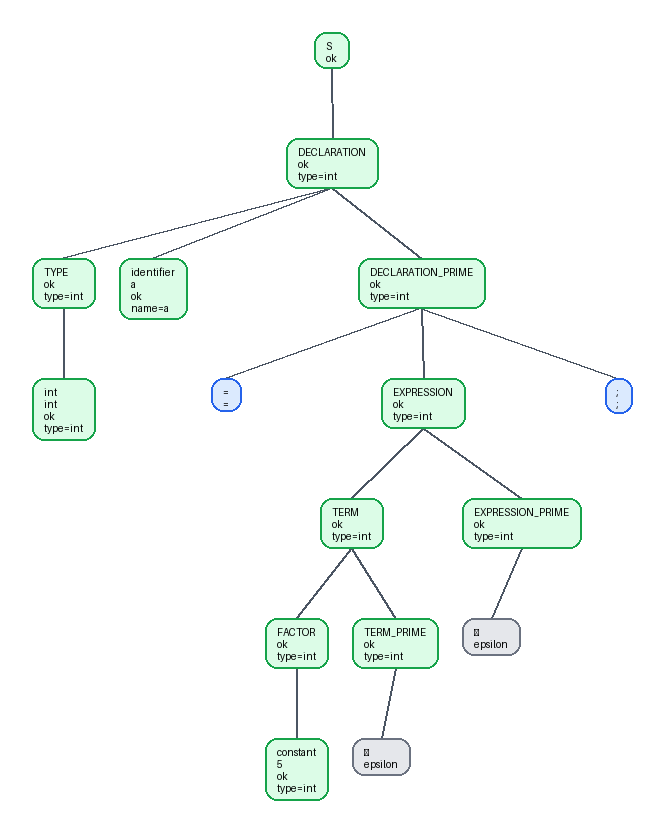
\includegraphics[width=0.55\linewidth]{verified_parse_tree.png}
    \caption{Verified parse tree from Test 1}
    \label{fig:test1input}
\end{figure}

\begin{figure}[H]
    \centering
    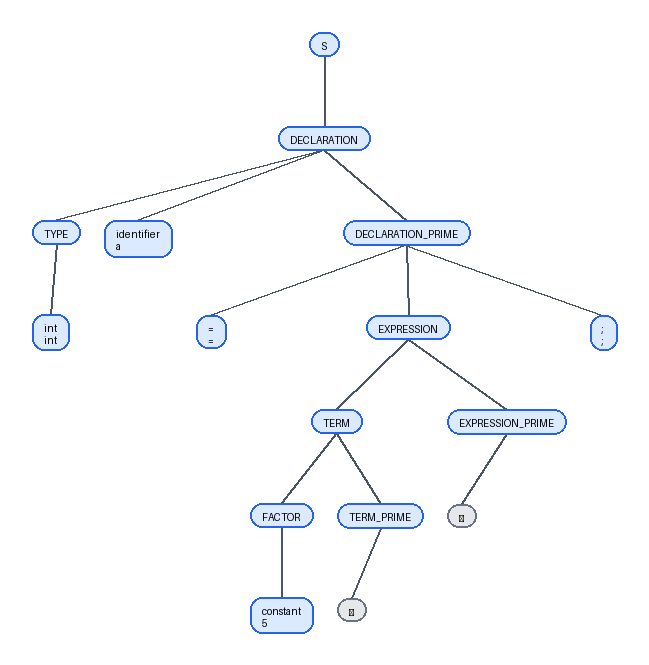
\includegraphics[width=0.75\linewidth]{parse_tree.png}
    \caption{Parse tree}
    \label{fig:parsetree}
\end{figure}

\begin{figure}[H]
    \centering
    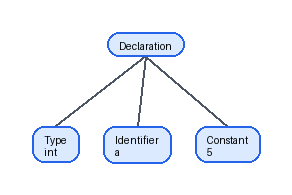
\includegraphics[width=0.75\linewidth]{abstract_tree.png}
    \caption{Abstract tree}
    \label{fig:abstracttree}
\end{figure}


\subsection{Test 2: Valid Arithmetic Expression}

\textbf{Input:} \texttt{int result = (3 + 5) * 2;}

\textbf{Result:}
\begin{verbatim}
Parsing Success!
SDT Verified!
\end{verbatim}

The expression \texttt{(3 + 5) * 2} is correctly parsed using the extended
arithmetic grammar. Type inference yields \texttt{int}, which is compatible with
the declared type.

\begin{figure}[H]
    \centering
    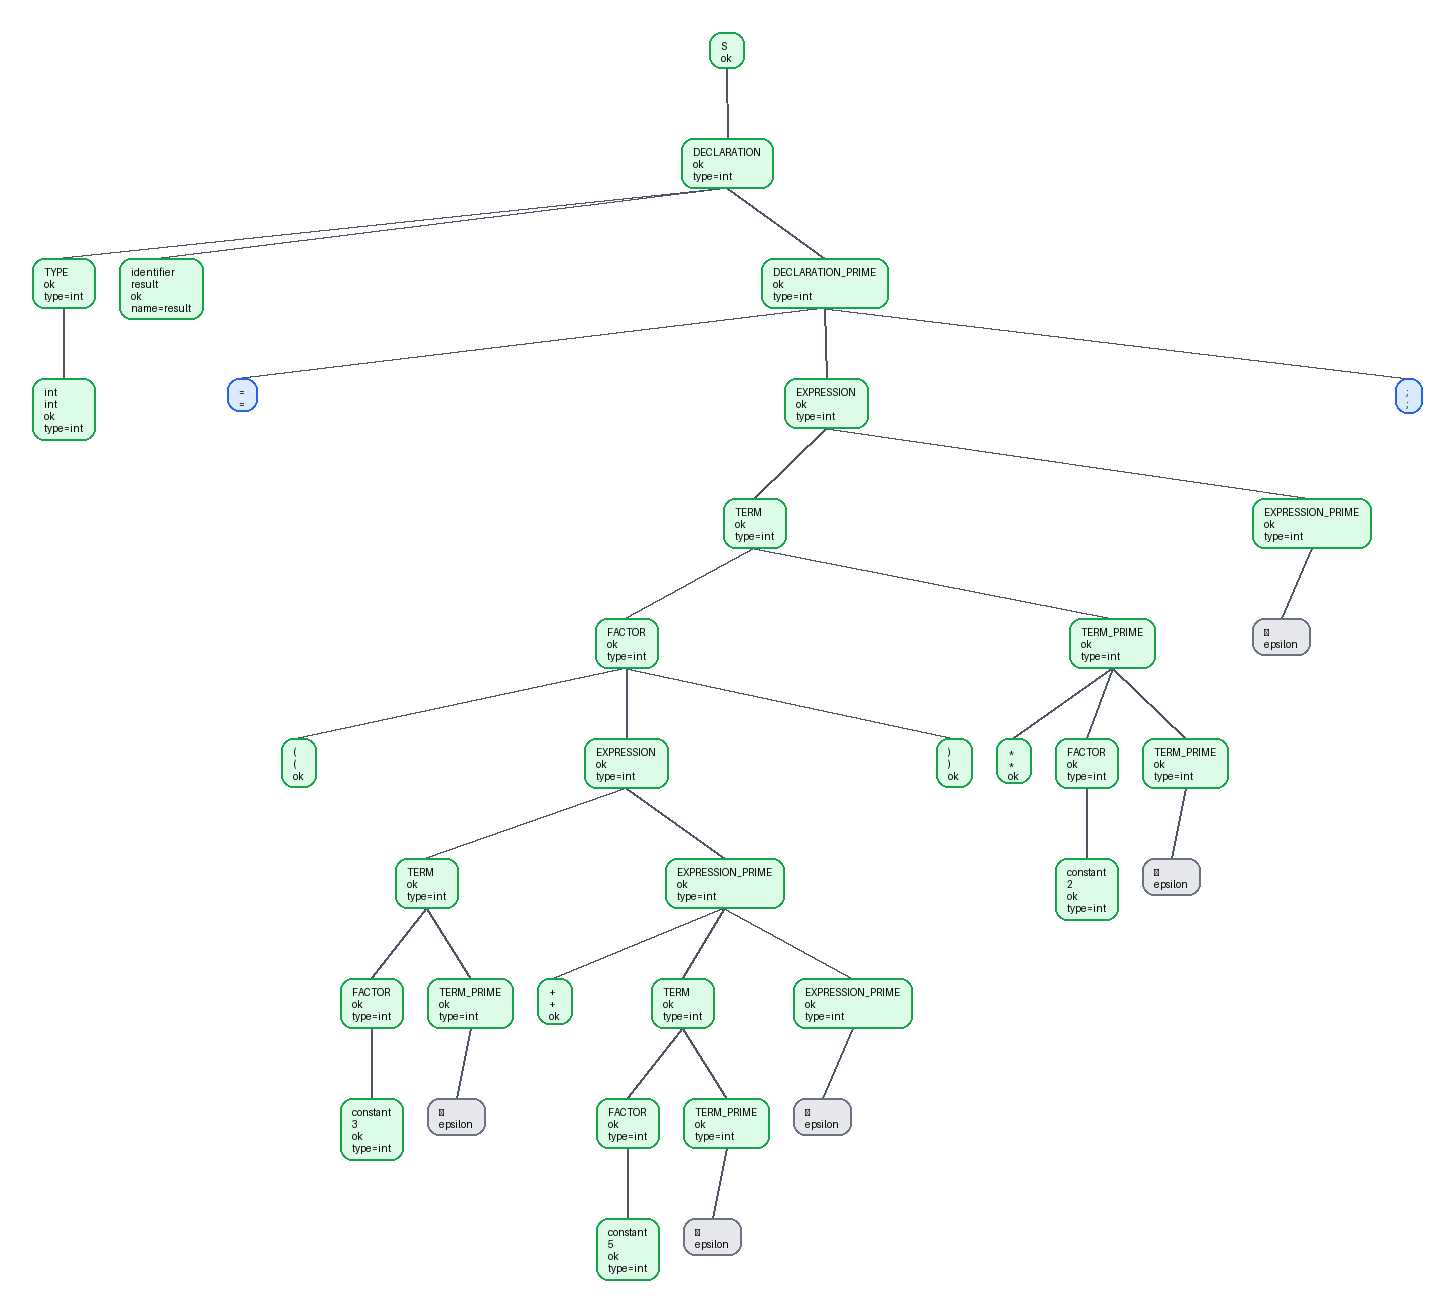
\includegraphics[width=0.55\linewidth]{verified_parse_tree2.png}
    \caption{Verified parse tree from Test 2}
    \label{fig:test1input}
\end{figure}

\begin{figure}[H]
    \centering
    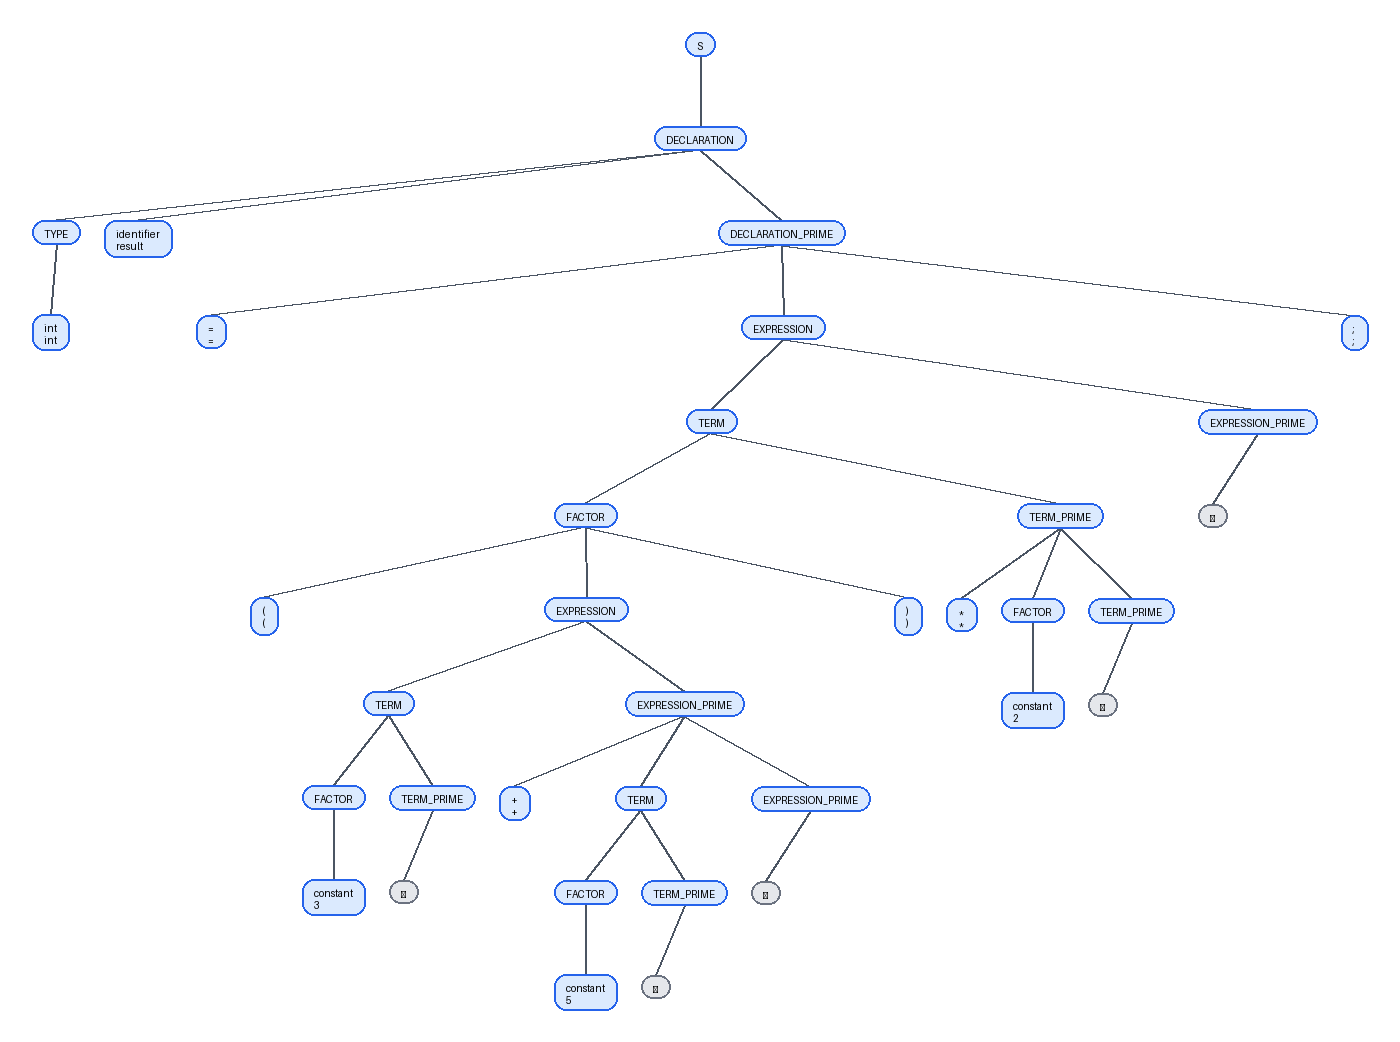
\includegraphics[width=0.75\linewidth]{parse_tree2.png}
    \caption{Parse tree}
    \label{fig:parsetree}
\end{figure}

\begin{figure}[H]
    \centering
    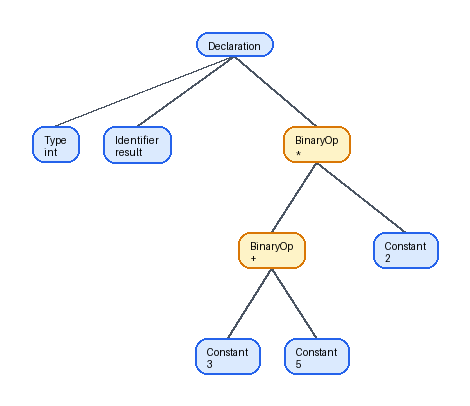
\includegraphics[width=0.75\linewidth]{abstract_tree2.png}
    \caption{Abstract tree}
    \label{fig:abstracttree}
\end{figure}


\subsection{Test 3: Semantic Error}

\textbf{Input:} \texttt{int x = y + 1;}

\textbf{Result:} Parse succeeds; SDT fails because identifier \texttt{y} was used
without a prior declaration. The verified parse tree marks the corresponding node
in red and records the semantic error message.

\begin{figure}[H]
    \centering
    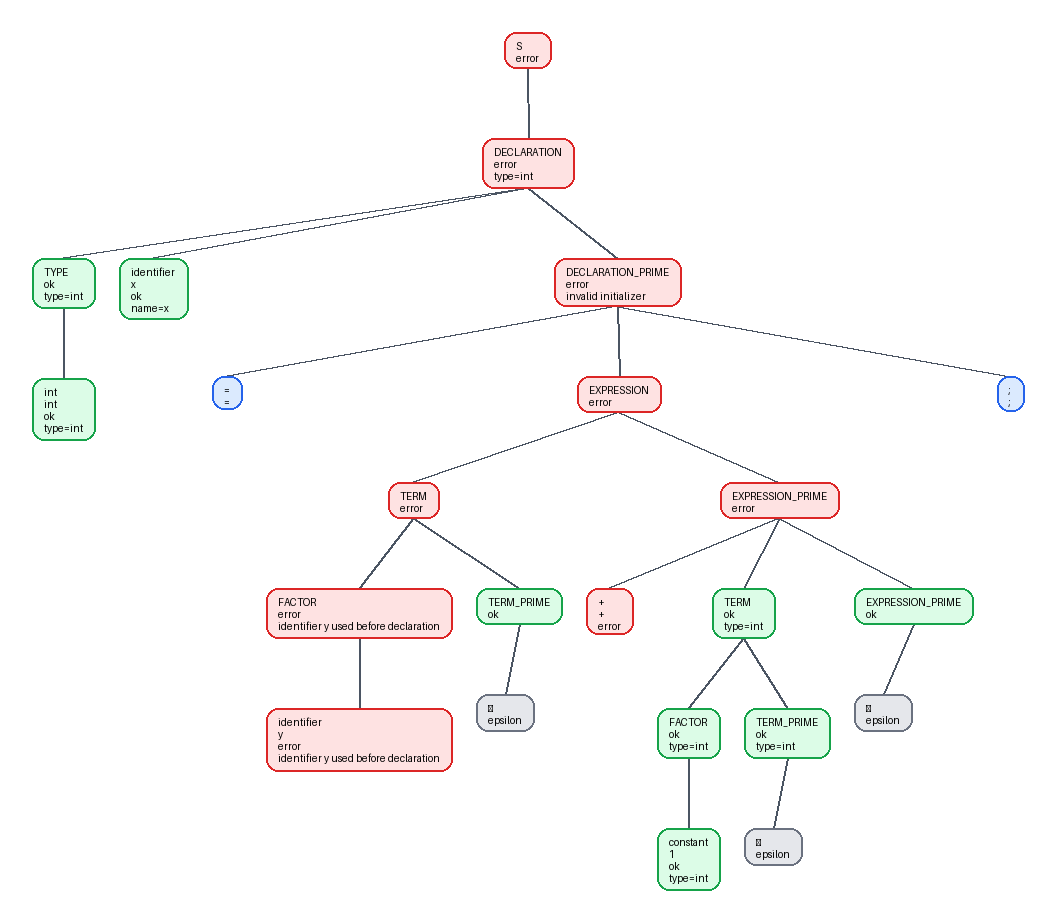
\includegraphics[width=0.55\linewidth]{verified_parse_tree3.png}
    \caption{Verified parse tree from Test 3}
    \label{fig:test1input}
\end{figure}

\begin{figure}[H]
    \centering
    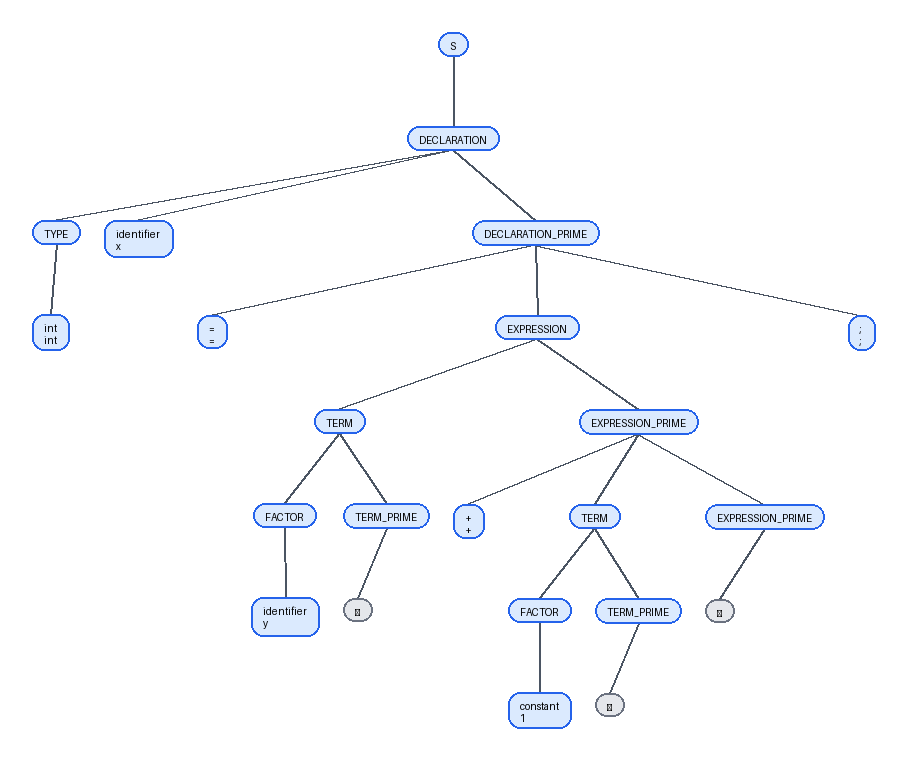
\includegraphics[width=0.75\linewidth]{parse_tree3.png}
    \caption{Parse tree}
    \label{fig:parsetree}
\end{figure}

\begin{figure}[H]
    \centering
    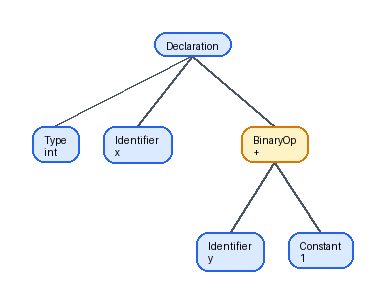
\includegraphics[width=0.75\linewidth]{abstract_tree3.png}
    \caption{Abstract tree}
    \label{fig:abstracttree}
\end{figure}

\subsection{Test 4: Syntax Error}

\textbf{Input:} \texttt{int x = ;}

\textbf{Result:} The parser fails when it encounters \texttt{;} where an expression
is expected. The SDT is not executed. The parse trace records the exact step at
which the error was detected.

\begin{figure}[H]
    \centering
    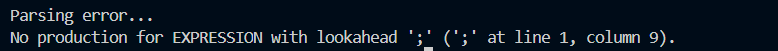
\includegraphics[width=0.55\linewidth]{error.png}
    \caption{Error from Test 4}
    \label{fig:test1input}
\end{figure}

\subsection{Generated Output Files}

Each successful execution writes the following files to \texttt{outputs/}:

\begin{table}[H]
\centering
\begin{tabular}{|l|l|}
\hline
\textbf{File} & \textbf{Description} \\
\hline
\texttt{first\_follow.txt}       & FIRST and FOLLOW sets for all grammar symbols \\
\hline
\texttt{parsing\_table.txt}      & Full LL(1) parsing table \\
\hline
\texttt{parse\_trace.txt}        & Step-by-step parsing trace \\
\hline
\texttt{parse\_tree.png}         & Complete parse tree with all productions \\
\hline
\texttt{verified\_parse\_tree.png} & Annotated parse tree with semantic state per node \\
\hline
\texttt{abstract\_tree.png}      & Compact AST with only semantically relevant nodes \\
\hline
\end{tabular}
\caption{Output artifacts generated by the pipeline}
\end{table}

The visual conventions used in the verified parse tree are:
\textbf{green} for valid nodes, \textbf{red} for semantic errors, \textbf{grey}
for epsilon nodes, \textbf{blue} for structural nodes without a semantic annotation,
and \textbf{yellow} for binary operator nodes in the AST.

%-----------------------------------------------------------------------
\section{Conclusions}

The implementation of a manual LL(1) parser and SDT in Python demonstrated that
building each compiler front-end component from first principles provides a clear
and practical understanding of syntactic and semantic analysis. By explicitly
computing FIRST and FOLLOW sets, constructing the parsing table, performing
stack-based parsing, and evaluating semantic rules, the project made visible the
full decision process followed by a predictive parser.

The resulting system successfully integrates lexical input, syntactic validation,
semantic verification, and structural representation through the generation of a
parse tree, a verified parse tree, and an Abstract Syntax Tree (AST). The project satisfies the objective of distinguishing among syntactically
and semantically correct inputs, syntactically correct but semantically invalid
inputs, and syntactically invalid inputs.

Beyond its functional outcome, the project also reinforced the theoretical
relationship between formal grammars, LL(1) parsing, and Syntax-Directed
Translation. Implementing these mechanisms manually, rather than relying on
external parsing tools, helped clarify how compiler front-end stages interact and why semantic analysis must be treated as a distinct phase from syntax checking.

The project have limitations, among this are support for only a single declaration per execution and the absence of relational operators, boolean expressions, nested scopes, and function definitions. These limitations can be work, such as extending the grammar, enriching the semantic rules, and incorporating additional language constructs to have a more complete compiler.

%-----------------------------------------------------------------------
\section{References}

\noindent [1] IBM, ``What is a compiler?,'' \textit{IBM Think}, [Online].\\
Available: \url{https://www.ibm.com/mx-es/think/topics/compiler}.
[Accessed: Mar. 2026].

\vspace{6pt}
\noindent [2] Wikipedia, ``LL parser,'' \textit{Wikipedia, The Free
Encyclopedia}, [Online].\\
Available: \url{https://en.wikipedia.org/wiki/LL_parser}.
[Accessed: Apr. 2026].

\vspace{6pt}
\noindent [3] GeeksforGeeks, ``Construction of LL(1) Parsing Table,''
\textit{GeeksforGeeks}, [Online].\\
Available: \url{https://www.geeksforgeeks.org/construction-of-ll1-parsing-table/}.
[Accessed: Apr. 2026].

\vspace{6pt}
\noindent [4] GeeksforGeeks, ``Syntax directed translation in compiler design,''
\textit{GeeksforGeeks}, [Online].\\
Available: \url{https://www.geeksforgeeks.org/syntax-directed-translation-in-compiler-design/}.
[Accessed: Apr. 2026].

\vspace{6pt}
\noindent [5] Wikipedia, ``Abstract syntax tree,'' \textit{Wikipedia, The Free
Encyclopedia}, [Online].\\
Available: \url{https://en.wikipedia.org/wiki/Abstract_syntax_tree}.
[Accessed: Apr. 2026].

\vspace{6pt}
\noindent [6] A. V. Aho, M. S. Lam, R. Sethi, and J. D. Ullman,
\textit{Compilers: Principles, Techniques, and Tools}, 2nd~ed.
Upper Saddle River, NJ, USA: Pearson Addison-Wesley, 2006.

\vspace{6pt}
\noindent [7] K. D. Cooper and L. Torczon,
\textit{Engineering a Compiler}, 2nd~ed.
Burlington, MA, USA: Morgan Kaufmann, 2011.



\end{document}